\documentclass[a4paper,14pt]{article}

\usepackage{comment} % Para comentar várias linhas ao mesmo tempo

%matemática
\usepackage{amsmath}
\usepackage{amssymb}

%diagramação
\usepackage{extsizes}
\everymath{\displaystyle}
\usepackage{geometry}
\usepackage{fancyhdr}
\usepackage{multicol}
\usepackage{graphicx}
\usepackage[brazil]{babel}
\usepackage[shortlabels]{enumitem}
\usepackage{cancel}
\usepackage{textcomp}
\usepackage{tcolorbox}

%tabelas
\usepackage{array} % Para melhor formatação de tabelas
\usepackage{longtable}
\usepackage{booktabs}  % Para linhas horizontais mais bonitas
\usepackage{float}   % Para usar o modificador [H]
\usepackage{caption} % Para usar legendas em tabelas
\usepackage{wrapfig} % Para usar tabelas e figuras flutuantes
\usepackage{xcolor} % Para cores do fundo de tabelas
\usepackage{colortbl} % Para cores do fundo de tabelas

%tikzpicture
\begin{comment}
	\usepackage{tikz}
	\usepackage{scalerel}
	\usepackage{pict2e}
	\usepackage{tkz-euclide}
	\usetikzlibrary{calc}
	\usetikzlibrary{patterns,arrows.meta}
	\usetikzlibrary{shadows}
	\usetikzlibrary{external}
\end{comment}


%pgfplots
\usepackage{pgfplots}
\pgfplotsset{compat=newest}
\usepgfplotslibrary{statistics}
\usepgfplotslibrary{fillbetween}

%colours
\usepackage{xcolor}



\columnsep=2cm
\hoffset=0cm
\textwidth=8cm
\setlength{\columnseprule}{.1pt}
\setlength{\columnsep}{2cm}
\renewcommand{\headrulewidth}{0pt}
\geometry{top=1in, bottom=1in, left=0.7in, right=0.5in}

\pagestyle{fancy}
\fancyhf{}
\fancyfoot[C]{\thepage}

\begin{document}
	
	\noindent\textbf{6FMA134 - Matemática} 
	
	\begin{center}Revisão: inteiros (Versão estudante)
	\end{center}
	
	\noindent\textbf{Nome:} \underline{\hspace{10cm}}
	\noindent\textbf{Data:} \underline{\hspace{4cm}}
	
	%\section*{Questões de Matemática}
	
	\begin{multicols}{2}
	    \noindent Operações com inteiros:
	    \begin{itemize}
	    	\item \textbf{Adição e subtração:} utilizar a reta orientada.
	    	\item \textbf{Multiplicação e divisão: }
	    	\begin{itemize}[label=\scalebox{0.5}{$\blacksquare$}]
	    		\item positivo com positivo é positivo;
	    		\item positivo com negativo é negativo;
	    		\item negativo com positivo é negativo;
	    		\item negativo com negativo é positivo.
	    	\end{itemize}
	    	\item Potenciação:
	    	\begin{itemize}[label=\scalebox{0.5}{$\blacksquare$}]
	    		\item $a^0 = 1$
	    		\item $a^n = a^{n - 1} \cdot a,$ se $n \geq 1$  
	    		\item $a^m \cdot a^n = a^{m + n}$
	    		\item $\frac{a^m}{a^n} = a^{m - n}$
	    		\item $a^m \cdot b^m = (a \cdot b)^m$
	    		\item $(a^m)^n = a^{m \cdot n}$
	    		\item $a^{m^n} = a^{(m^{n})}$
	    	\end{itemize}
	    \end{itemize}
		\noindent\textsubscript{--------------------------------------------------------------------------}
		\begin{enumerate} 
			\item Representar na reta:
			\begin{enumerate}[a)] 
				\item x + 6 \\
				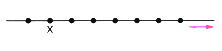
\includegraphics[width=1\linewidth]{6FMA134_imagens/imagem1}
				\item y - 7 \\
				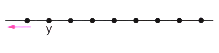
\includegraphics[width=1\linewidth]{6FMA134_imagens/imagem2}
				\item m + 0 \\
				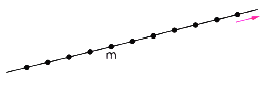
\includegraphics[width=1\linewidth]{6FMA134_imagens/imagem3}
			\end{enumerate}
			\item Assinale \textbf{V} (verdadeiro) ou \textbf{F} (falso) para quaisquer inteiros $a, b$ e $c$.
			\begin{enumerate}[a)] 
				\item (~~) $(a + b)c = ac + bc$
				\item (~~) $a + b \in \mathbb{Z}$
				\item (~~) $a + (b + c) = (a + b) + c$
				\item (~~) $a + (-a) = 0$
				\item (~~) $a + (b \cdot c) = (a + b) \cdot (a + c)$
				\item (~~) $a + b = b + a$
			\end{enumerate}
			\item Escreva na forma $a^n$. Suponha $w, t, z \neq 0$.
			\begin{enumerate}[a)] 
				\item $(-23)^7 \cdot (-23)^9$ \\\\\\
				\item $z^{32} \cdot z^{26}$ \\\\\\
				\item $\frac{9^9}{9^5}$ \\\\\\
				\item $\frac{(-w)^6}{(-w)^3}$ \\\\\\
				\item $\frac{5^3 \cdot 5^2 \cdot 5^5}{5^4 \cdot 5^6 \cdot 5^7}$ \\\\\\
				\item $\frac{t^6 \cdot t^27 \cdot t^{-5}}{t^{18} \cdot t^7 \cdot t^6}$ \\\\\\
				\item $3^9 \cdot (-2)^9 \cdot 7^9 \cdot (-9)^9$ \\\\\\
				\item $6^{4^3}$ \\\\\\
				\item $\frac{z^7 \cdot z^{2^3} \cdot z \cdot z^5}{z^9 \cdot z \cdot z^6}$ \\\\\\
			\end{enumerate}
			%37 a 44
			\item Efetuar:
			\begin{enumerate}[a)]
				\item -72 + 94 - 31 + 26 \\\\\\\\\\\\\\\\
				\item -5 + 1 - 9 + 7 - 2 - 13 \\\\\\\\\\\\
				\item -23 + 4 - 8 - 32 - 12 + 86 \\\\\\\\\\\\
				\small \item 1 + 3 - 4 + 8 - 9 + 6 - 52 + 31 \\\\\\\\\\\\
				\normalsize \item 5 + 7 - 23 + 14 - 13 \\\\\\\\\\\\
				\item 4 + 2 - 3 + 8 - 12 \\\\\\\\\\\\
				\item -9 + 15 - 12 + 3 - 2 \newpage
				\item 8 - 120 + 15 - 95 + 78 \\\\\\\\\\\\
			\end{enumerate}
			\item Pela manhã, o termômetro indicava -8 °C; ao meio-dia, a temperatura havia subido em 10 °C; e, no fim da tarde, a temperatura havia subido em 10 °C; e, no fim da tarde, a temperatura caiu em 5 °C.
			\begin{enumerate}[a)]
				\item Represente, usando adição e subtração, a temperatura no final da tarde. \\\\\\\\\\\\\\\\\\\\
				\item Qual foi a temperatura indicada pelo termômetro no fim da tarde? \\\\\\\\\\\\\\\\\\
			\end{enumerate}
			\item Amanda está jogando um jogo em seu computador. Se ela ganhar uma partida, ela ganha cinco pontos e, se perder, perde um ponto. Amanda ganhou 12 partidas e perdeu 8. Represente, usando adição e multiplicação, o número de pontos de Amanda no final do jogo. Com quantos pontos Amanda ficou no final? \\\\\\\\\\\\\\\\\\\\\\\\\\\\
			\item Calcular:
			\begin{enumerate}[a)]
				\item $(3a + 2b)(2a + b)$ \\\\\\\\\\
				\item $(x - 3z)^2$ \newpage
				\item $(1 + 3a)(2 + b)$ \\\\\\\\\\
				\item $(a + b) \cdot (a - b)$ \\\\\\\\\\
				\item $(2w + t)^2$ \\\\\\\\\\
			\end{enumerate}
			\item Efetuar:
			\begin{enumerate}[a)]
				\item $8 - 2 \cdot 7 + 13 \cdot 3$ \\\\\\\\\\\\\\\\\\
				\item $6 + 5 \cdot 3 - 8 \cdot 2 - 3^2$ \\\\\\\\\\\\\\\\\\
				\item $(-2)^3 \cdot 3 + 4 \cdot 5 \cdot 3^2 - 42 : 6$ \\\\\\\\\\\\\\
				\item $21 \cdot 3^0 + 7 - 2 \cdot 5^2 + (54 - 6) : 8$ \\\\\\\\\\\\\\
			\end{enumerate}
			\item Tem-se dois tipos de extrato bancário, um para o cliente e outro para o banco (extrato interno). Diferentemente daquele que é fornecido ao cliente, o banco registra, para cada operação bancária, o oposto de que registra, no extrato do cliente. Assim, se Fernanda deposita R\$ 1.000,00, no extrato dela aparece -1.000,00, significando que o banco tem em seu poder uma quantia que não é sua. Observe que, em ambos os extratos, para obter o saldo em conta-corrente, é preciso somar os números que representam as operações anteriores até o último saldo em conta-corrente. \\
			Preencha a seguir os dois extratos dos dias 10, 11 e 12.
			\\
			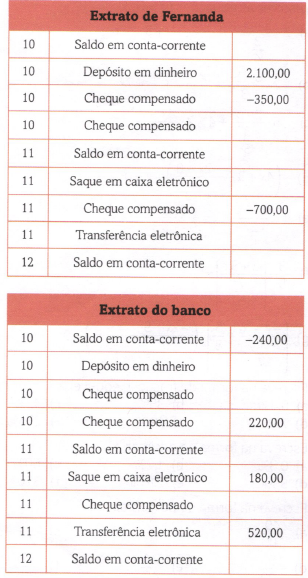
\includegraphics[width=1\linewidth]{6FMA134_imagens/imagem4}
			\item Efetuar:
			\begin{enumerate}[a)]
				\item $(-12) \cdot 25$ \\\\\\\\\\
				\item $(-15)(-13)$ \\\\\\\\\\\\\\\\\\\\\\
				\small \item $97^2$ (dica: $(a - 3)^2 = a^2 - 6a + 9$) \\\\\\\\\\\\\\\\\\
				\normalsize \item $-32 \cdot 16$ \\\\\\\\\\\\\\\\\\
				\item $(9 999 + 9 999) \cdot 25$ \\\\\\\\\\\\\\\\\\
				\item $4 001 \cdot 3 999$ (dica: $(a + 1) \cdot (a - 1) = a^2 - 1 $) \newpage
				\item Efetuar:
				\begin{enumerate}[a)]
					\item $(-7)^4$  \\\\\\\\\\\\\\\\\\
					\item $-4^2 + (-3)^3$ \\\\\\\\\\\\\\\\\\
					\item $-(-6)^2 + (-2)^3 + 5^3$ \\\\\\\\\\\\\\\\\\
					\item $-4^0 + 9^2 -(-4)^3 + 3^4$ \\\\\\\\\\\\\\\\\\
					\item $-6 + (3^2(-4 + 9) + 2^3) \cdot 4 - 7 + 4 \cdot 1$ \\\\\\\\\\\\\\\\\\
					\item $(-4)(-1)^4 + ((1 + 4) \cdot 2 -(-7)^2 + 9)$ \\\\\\\\\\\\\\\\\\
				\end{enumerate}
			\end{enumerate}
		\end{enumerate}
		$~$ \\ $~$ \\ $~$ \\ $~$ \\ $~$ \\ $~$ \\ $~$ \\ $~$ \\ $~$ \\ $~$ \\ $~$ \\ $~$ \\ $~$ \\ $~$ \\ $~$ \\ $~$ \\ $~$ \\ $~$
	\end{multicols}
\end{document}